\section{Tracking und Stabilisierung der Kugelpositionen}
Das in Abschnitt \ref{kap:tracking} beschriebene Tracking zur Stabilisierung der Kugelpositionen hat zu einer deutlichen,
visuellen Verbesserung der Live-Detektion und -Anzeige geführt.
Sofern der Spielstand ruhig ist, also keine Kugeln in Bewegung sind, bewegen sich die
projizierten Kreise rund um die detektierte Position kaum noch.
Ohne Tracking ist das Rauschen in der detektierten Position anhand der bewegenden Kreise sichtbar.

Diese visuelle Verbesserung kann auch statistisch quantifiziert werden, indem die Detektion auf einem Video eines
ruhigen Spielstandes durchgeführt wird. Die Detektion kann auf jedem einzelnen Frame des Videos durchgeführt werden, und
die detektierte Position mit derjenigen im vorherigen Frame verglichen werden.
Die Distanz zwischen der detektierten Position in Frame $F_{t-1}$ und derjenigen in Frame $F_{t}$ bildet anschliessend
eine Messung, die gesammelt wird.

Auf den gesammelten Distanzen können anschliessend statistische Kennzahlen berechnet werden.
Diese Messungen wurden mit und ohne Stabilisierung der Kugelpositionen durchgeführt, die Resultate sind in Tabelle \ref{tab:detektion_resultate_tracking_stats} aufgeführt.
Die Messungen basieren auf einem Videoausschnitt von 178 Frames eines Videos mit einem Spielstand wo 21 Kugeln stillstehen.
Die Messung wurde erst nach 30 Frames gestartet, damit die Messung mit eingeschalteter Stabilisierung bereits einige
Daten sammeln konnte.
Während dieser Aufwärmphase wäre die Detektion mit eingeschalteter Stabilisierung anfällig auf Rauschen in der Detektion,
wie es die Detektion ohne Stabilisierung ist.
Durch diesen Vorlauf von 30 Frames beträgt der gemessene Videoausschnitt 148 Frames.
Dies resultiert in $148 \cdot 21 = 3108$ Messwerten.
Aus Tabelle \ref{tab:detektion_resultate_tracking_stats} wird klar, dass die Stabilisierung die Bewegung der
detektierten Kugelpositionen deutlich verringern konnte.

\begin{table}[ht]
    \rowcolors{1}{\seccolor!10}{\seccolor!10} % Rows with 10% of secondary color
    \begin{tabular}{ lrr }
        \rowcolor{\seccolor!50}
        Bezeichnung & Stabilisierung ausgeschaltet & Stabilisierung eingeschaltet\\
        Anzahl Messwerte & 3108 & 3108\\
        Minimum & 0mm & 0mm\\
        Unteres Quartil $Q_{0.25}$ & 1.638916mm & 0.081972mm\\
        Median $Q_{0.5}$ & 2.359856mm & 0.129632mm\\
        Oberes Quartil $Q_{0.75}$ & 3.714067mm & 0.222898mm\\
        Quartilabstand $Q_{0.75} - Q_{0.25}$ & 2.075151mm & 0.140926mm\\
        Maximum & 13.590104mm & 4.043161mm\\
        Summe aller Messungen & 7654.91mm & 588.849mm
    \end{tabular}
    \caption{
        Statistische Zahlen zu der Verteilung der Veränderung der detektierten Kugelpositionen über eine Dauer von
        148 Video-Frames mit und ohne Stabilisierung.
        Bei einem Messwert handelt es sich um die Distanz zwischen der detektierten Kugelposition in Frame $F_{t-1}$
        und Frame $F_{t}$ für eine Kugel.
    }
    \label{tab:detektion_resultate_tracking_stats}
\end{table}
% ohne stabilisierung: Total delta movement summary: count=3108 min=0.000000, lower quartile=1.638916, median=2.359856, upper quartile=3.714067, max=13.590104
% mit  stabilisierung: Total delta movement summary: count=3108 min=0.000000, lower quartile=0.081972, median=0.129632, upper quartile=0.222898, max=4.043161
% ohne stabilisierung: Total delta movement: 7654.91mm, 148 frames, lost: 0
% mit  stabilisierung: Total delta movement: 588.849mm, 148 frames, lost: 0

In Abbildung \ref{fig:detektion_resultate_tracking_boxplot} sind die Daten aus Tabelle \ref{tab:detektion_resultate_tracking_stats}
in zwei Box-Plot-Diagrammen visualisiert.

\begin{figure}[h!]
    \begin{center}
        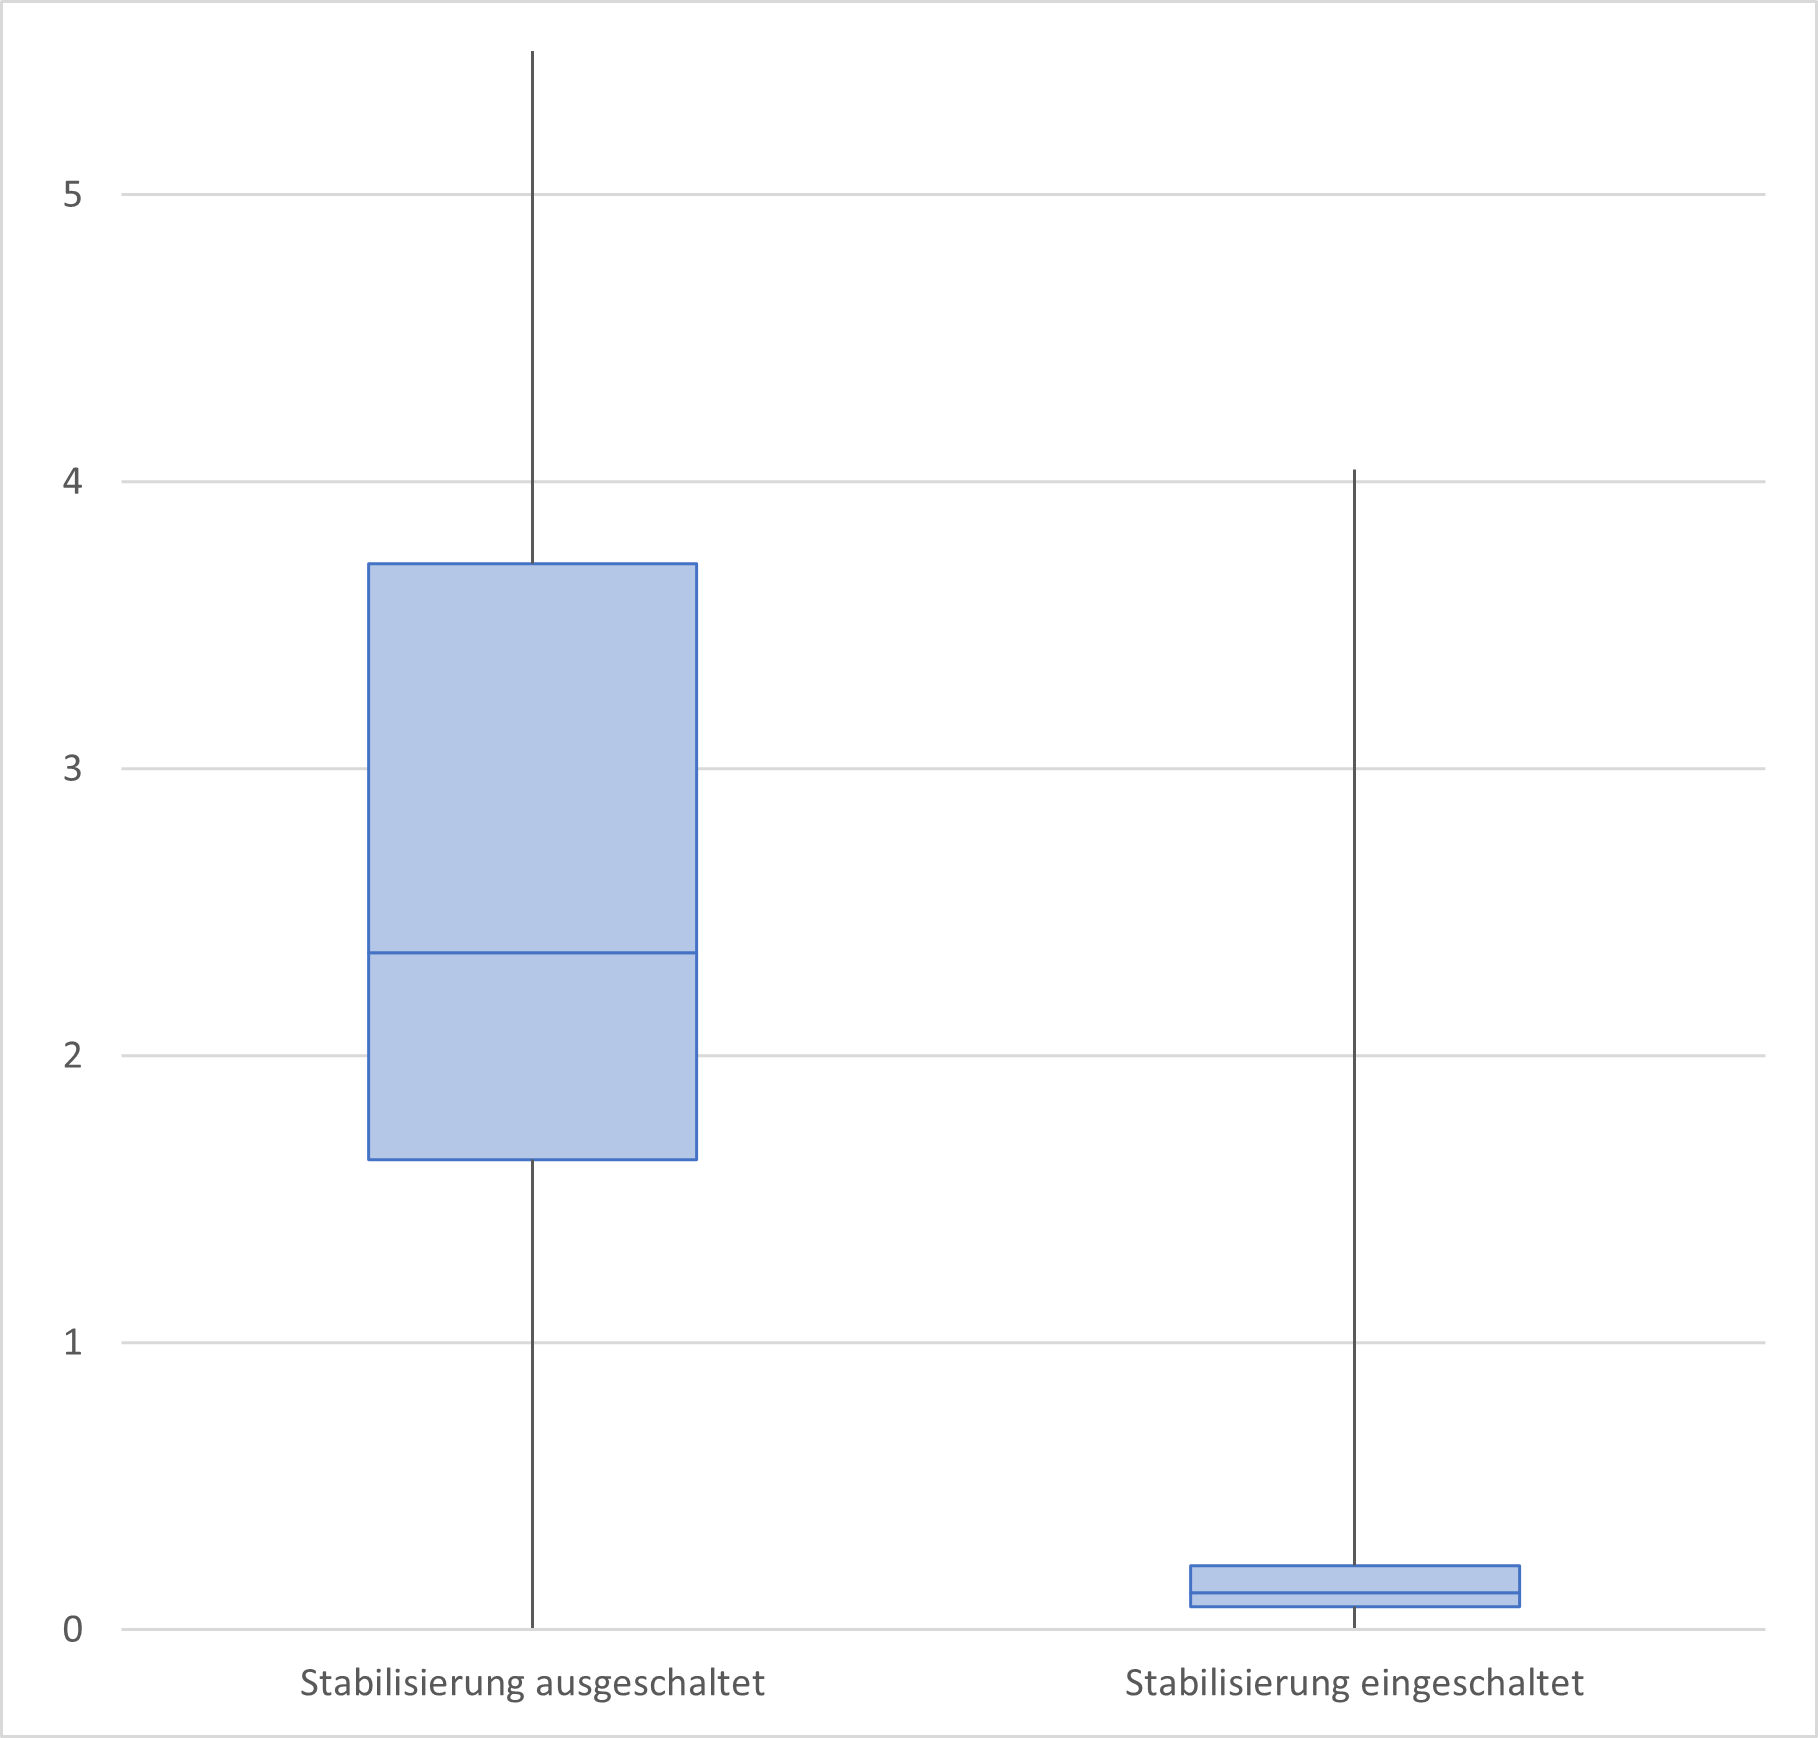
\includegraphics[width=0.5\linewidth]{../common/04_results/resources/stabilisierung_boxplot.png}
    \end{center}
    \caption{
        Box-Plot-Diagramme zu der Bewegung der Kugelpositionen mit und ohne Stabilisierung
        gemäss Tabelle \ref{tab:detektion_resultate_tracking_stats}.
        Der Wertebereich der Y-Achse wurde auf 5 beschränkt, damit das rechte Diagramm ersichtlich ist.
        Die Antenne des linken Diagrammes geht bis zum Maximum von 13.59mm.
    }
    \label{fig:detektion_resultate_tracking_boxplot}
\end{figure}
